\documentclass[border=10pt]{standalone}
\usepackage{tikz}
\usetikzlibrary{arrows.meta, calc, shadings, patterns}

\begin{document}
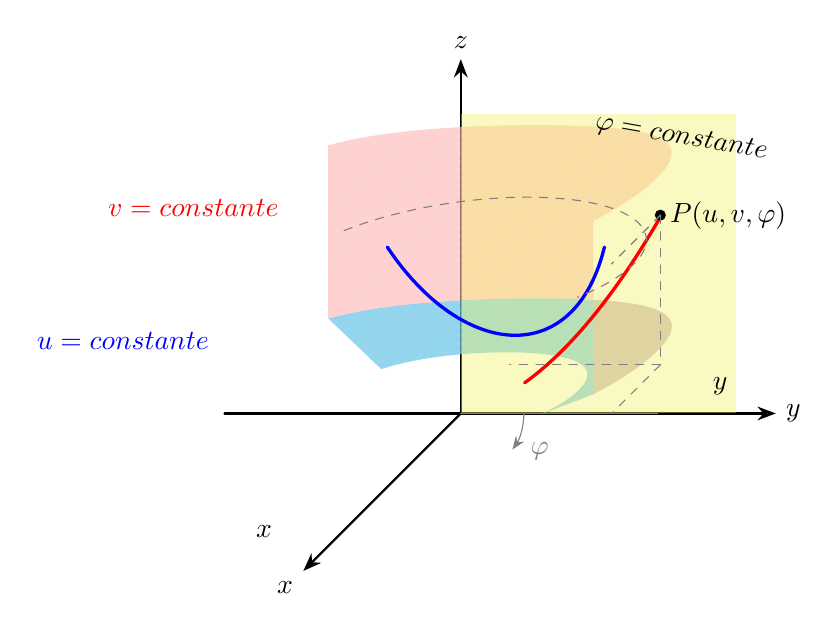
\begin{tikzpicture}[>=Stealth, line join=round, line cap=round]
  
  % Define colors
  \definecolor{surfaceblue}{RGB}{100,200,230}
  \definecolor{surfacepink}{RGB}{255,180,180}
  \definecolor{phiplane}{RGB}{240,240,100}
  
  % Draw axes
  \draw[thick, ->] (-3,-1,0) -- (4,-1,0) node[right] {$y$};
  \draw[thick, ->] (0,-1,0) -- (0,3.5,0) node[above] {$z$};
  \draw[thick, ->] (0,-1,0) -- (-2,-3,0) node[below left] {$x$};
  
  % Draw x-axis label
  \node at (-2.5,-2.5,0) {$x$};
  
  % Draw phi angle in xy-plane
  \draw[gray] (0,-1,0) -- (2.5,-1,0);
  \draw[gray, ->] (0.8,-1,0) arc (0:-35:0.8) node[midway, below right] {$\varphi$};
  
  % Draw lower part of surface (blue)
  \fill[surfaceblue, opacity=0.7] 
    plot[domain=-150:30, smooth] ({2.5*cos(\x)}, {-1 + 0.8*(cos(\x))^2 + 0.5*(sin(\x))^2}, {2.5*sin(\x)})
    -- plot[domain=30:-150, smooth] ({1.5*cos(\x)}, {-1 + 0.3*(cos(\x))^2 + 0.2*(sin(\x))^2}, {1.5*sin(\x)})
    -- cycle;
  
  % Add hatching to lower surface
  \fill[pattern=north east lines, pattern color=blue!30, opacity=0.3]
    plot[domain=-150:30, smooth] ({2.5*cos(\x)}, {-1 + 0.8*(cos(\x))^2 + 0.5*(sin(\x))^2}, {2.5*sin(\x)})
    -- plot[domain=30:-150, smooth] ({1.5*cos(\x)}, {-1 + 0.3*(cos(\x))^2 + 0.2*(sin(\x))^2}, {1.5*sin(\x)})
    -- cycle;
  
  % Draw upper part of surface (pink)
  \fill[surfacepink, opacity=0.6] 
    plot[domain=-150:30, smooth] ({2.5*cos(\x)}, {-1 + 2.2 + 0.8*(cos(\x))^2 + 0.5*(sin(\x))^2}, {2.5*sin(\x)})
    -- plot[domain=30:-150, smooth] ({2.5*cos(\x)}, {-1 + 0.8*(cos(\x))^2 + 0.5*(sin(\x))^2}, {2.5*sin(\x)})
    -- cycle;
  
  % Add hatching to upper surface
  \fill[pattern=north east lines, pattern color=red!20, opacity=0.2]
    plot[domain=-150:30, smooth] ({2.5*cos(\x)}, {-1 + 2.2 + 0.8*(cos(\x))^2 + 0.5*(sin(\x))^2}, {2.5*sin(\x)})
    -- plot[domain=30:-150, smooth] ({2.5*cos(\x)}, {-1 + 0.8*(cos(\x))^2 + 0.5*(sin(\x))^2}, {2.5*sin(\x)})
    -- cycle;
  
  % Draw phi = constant plane (yellow)
  \fill[phiplane, opacity=0.4] 
    (0,-1,0) -- (3.5,-1,0) -- (3.5,2.8,0) -- (0,2.8,0) -- cycle;
  
  % Draw u = constant curve (blue)
  \draw[blue, very thick] 
    plot[domain=-140:-40, smooth, samples=30] ({1.8*cos(\x)}, {-1 + 0.5*(cos(\x))^2 + 0.3*(sin(\x))^2 + 0.05*(\x+90)^2/100}, {1.8*sin(\x)});
  
  % Draw v = constant curve (red)
  \draw[red, very thick] 
    plot[domain=0.8:2.5, smooth, samples=30] ({\x*cos(-40)}, {-1 + 0.3*\x^2}, {\x*sin(-40)});
  
  % Point P
  \coordinate (P) at (2.5*0.766, 0.9, 2.5*-0.643);
  \fill (P) circle (2pt);
  \node[right] at (P) {$P(u,v,\varphi)$};
  
  % Dashed projection lines
  \draw[dashed, gray] (P) -- (2.5*0.766, -1, 2.5*-0.643);
  \draw[dashed, gray] (2.5*0.766, -1, 2.5*-0.643) -- (2.5*0.766, -1, 0);
  \draw[dashed, gray] (2.5*0.766, -1, 2.5*-0.643) -- (0, -1, 2.5*-0.643);
  \draw[dashed, gray] (P) -- (2.5*0.766, 0.9, 0);
  
  % Horizontal dashed line at constant z
  \draw[dashed, gray] 
    plot[domain=-150:30, smooth] ({2.2*cos(\x)}, {0.9}, {2.2*sin(\x)});
  
  % Labels for coordinate curves
  \node[blue, left] at (-2.5, 0.5, 1.5) {$u = \text{constante}$};
  \node[red, left] at (-2, 1.8, 0.5) {$v = \text{constante}$};
  \node[rotate=-10] at (2.8, 2.5, 0) {$\varphi = \text{constante}$};
  
  % y label on axis
  \node[below right] at (2.5, -1, -1.5) {$y$};
  
\end{tikzpicture}
\end{document}